\documentclass[12pt]{article}
\setlength\parindent{0pt}
\usepackage{fullpage}
\usepackage[margin=0.5in]{geometry}
\usepackage{amsmath}
\usepackage{pdflscape}
\usepackage{graphicx}
\setlength{\parskip}{4mm}
\def\LL{\left\langle}   % left angle bracket
\def\RR{\right\rangle}  % right angle bracket
\def\LP{\left(}         % left parenthesis
\def\RP{\right)}        % right parenthesis
\def\LB{\left\{}        % left curly bracket
\def\RB{\right\}}       % right curly bracket
\def\PAR#1#2{ {{\partial #1}\over{\partial #2}} }
\def\PARTWO#1#2{ {{\partial^2 #1}\over{\partial #2}^2} }
\def\PARTWOMIX#1#2#3{ {{\partial^2 #1}\over{\partial #2 \partial #3}} }
\newcommand{\BE}{\begin{displaymath}}
\newcommand{\EE}{\end{displaymath}}
\newcommand{\BNE}{\begin{equation}}
\newcommand{\ENE}{\end{equation}}
\newcommand{\BEA}{\begin{eqnarray}}
\newcommand{\EEA}{\nonumber\end{eqnarray}}
\newcommand{\EL}{\nonumber\\}
\newcommand{\la}[1]{\label{#1}}
\newcommand{\ie}{{\em i.e.\ }}
\newcommand{\eg}{{\em e.\,g.\ }}
\newcommand{\cf}{cf.\ }
\newcommand{\etc}{etc.\ }
\newcommand{\Tr}{{\rm tr}}
\newcommand{\etal}{{\it et al.}}
\newcommand{\OL}[1]{\overline{#1}\ } % overline
\newcommand{\OLL}[1]{\overline{\overline{#1}}\ } % double overline
\newcommand{\OON}{\frac{1}{N}} % "one over N"
\newcommand{\OOX}[1]{\frac{1}{#1}} % "one over X"

\pagenumbering{gobble}

\begin{document}
\Large

\begin{center}
	Week 13, Day 2 \\
	Exercises on combining rotation and translation
	
	\large
	
	\medskip
	
	Exercise 1: Torque on a yo-yo
	
\end{center}

\normalsize

\begin{minipage}{0.6\textwidth}
A Yo-Yo consists of a cylinder of radius $R$ with a thin slit cut in it. Inside the slit is a smaller inner cylinder of radius $r$ with a string attached to it and then wound around the cylinder. Note that the moment of inertia of a cylinder of radius $R$ is $I=\frac{1}{2}mR^2$; since the slit in the Yo-Yo is so thin, you do not need to consider it in computing the moment of inertia. (Thus, both have the same moment of inertia: $I=\frac{1}{2}mR^2$.)

If a person holds the end of the string and drops the Yo-Yo, it will begin to spin as it falls, unwinding the string as it does. 

\bigskip\bigskip

a) Suppose that you have a red Yo-Yo with $r=0.1 R$ (that is, with a very small inner cylinder) and a blue Yo-Yo with $r=0.4 R$ (with a thicker inner cylinder). Using an argument based on energy, predict which one will fall faster when it is dropped, and describe why it will do so. \textit{(You shouldn't do any calculations here.)}
\end{minipage}
\begin{minipage}{0.20\textwidth}
	\begin{center}
		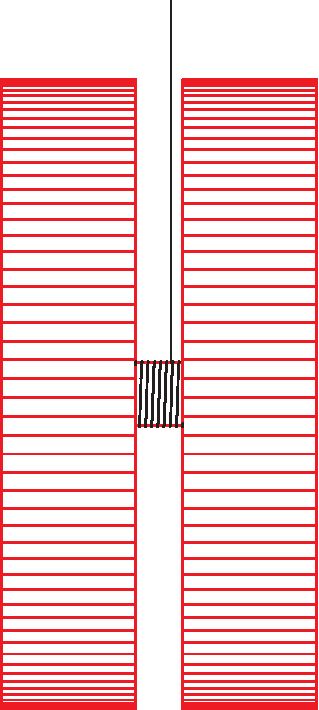
\includegraphics[width=0.7\textwidth]{red-crop.pdf}
		\end{center}
\end{minipage}
\begin{minipage}{0.20\textwidth}
		\begin{center}
		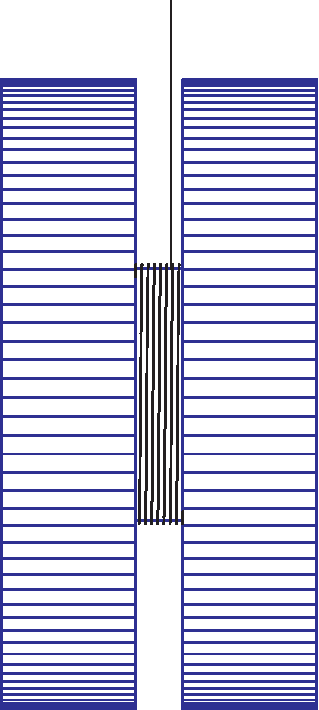
\includegraphics[width=0.7\textwidth]{blue-crop.pdf}
			\end{center}
\end{minipage}


\vspace{1.5in}

b) Now, you'll calculate the downward acceleration of the Yo-Yo. In this case, the Yo-Yo both {\it translates} and {\it rotates} as it does so.

Start by drawing an extended force diagram for the Yo-Yo, showing all the forces acting on it {\it and where they act}. (Think carefully about which perspective your force diagram should show -- it's not the one in the diagrams above.)

\vspace{2in}

\newpage

c) Since it both translates and rotates, you will need both $\vec F = m \vec a$ to relate the forces on it to its translational acceleration and $\tau = I \alpha$ to relate the torques on it to its linear acceleration. Construct both of these equations, using the forces that appear on your force diagram. \textit{(Hint: The tension in the string both applies a torque to the Yo-Yo and affects its translational acceleration.)}

\vspace{2.5in}

d) In the above two equations, you will have three unknowns: the tension in the string, the translational acceleration, and the angular acceleration $\alpha$. However, you can relate two of them to each other. What is that relation? \textit{(Hint: Think carefully about minus signs here!)}

\vspace{1in}

e) Now you should have enough information to solve for $a$ in terms of $g$, $r$, and $R$. Once you have a value for your acceleration, call your GTA or coach over and have them check your work. Discuss with them whether the red or blue Yo-Yo in part (a) would fall faster. 

\newpage

\begin{center}
	\large Exercise 2: a Ping-Pong ball on a table
\end{center}

Some people are playing Ping-Pong outdoors and have left a ball of mass $m$ on the table when a gentle breeze begins; this wind applies a constant horizontal force $F_w$ on the ball. The coefficient of static friction between the ball and the table is $\mu_s$, and the coefficient of kinetic friction is $\mu_k$. The Ping-Pong ball is a hollow shell and has a moment of inertia $\frac{2}{3}mr^2$.

\begin{enumerate}

\item Suppose first that the breeze is very gentle, so that the ball rolls smoothly on the table without slipping. If $F_w$ is very small, will the frictional force on the ball be $\mu_s mg$, $\mu_k mg$, or some other value $F_f$ that you don't know yet? Discuss this with your group and call your coach or TA over to join your conversation. {\it (Don't continue here until you've discussed this with one of your instructors.)}

\bigskip

\item Determine the ball's translational acceleration $a$ and angular acceleration $\alpha$ in terms of $F_w$ and $m$. (You will need to do all the usual things that you did during the last problem -- draw a force diagram, etc.) 

\newpage

\item Now, suppose that the wind steadily increases in strength. What is the largest wind force $F_w$ for which the ball will roll without slipping? {\it (What other force limits how strong the wind can be?)}


\vspace{4.5in}

\item Suppose that the wind becomes even stronger, so that the ball skids across the table. Now determine both its translational acceleration $a$ and its angular acceleration $\alpha$.
\end{enumerate}


\end{document}
